\documentclass[tikz]{standalone}
\usetikzlibrary{decorations.pathreplacing}
\usepackage{mathtools}
\DeclarePairedDelimiter{\abs}{\lvert}{\rvert}
\renewcommand{\epsilon}{\varepsilon}


\begin{document}

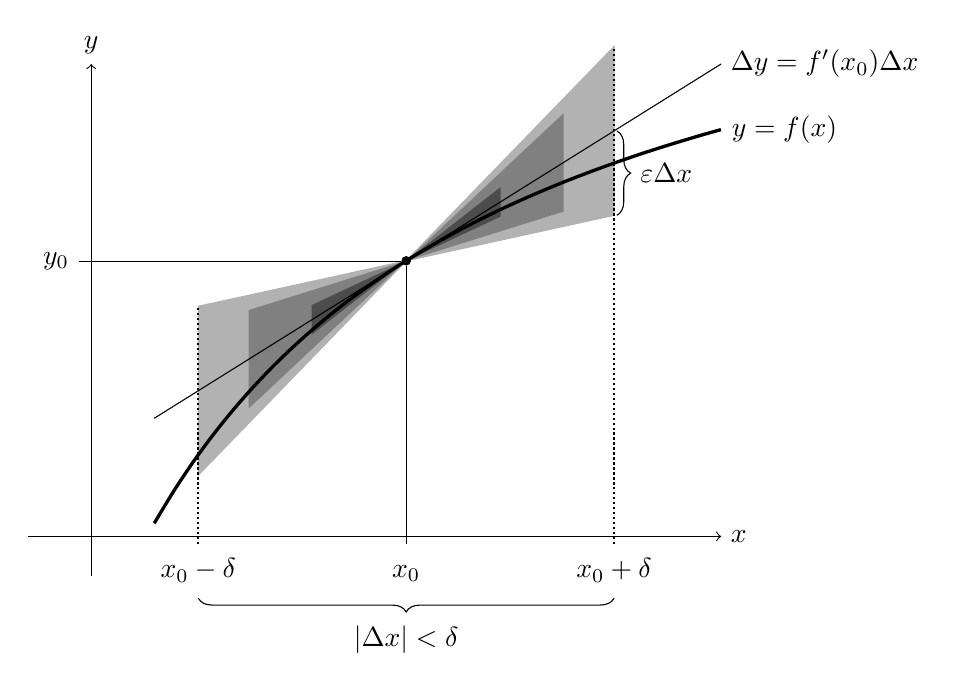
\begin{tikzpicture}[xscale=8,yscale=5]
    \newcommand{\xmin}{-.4} \newcommand{\xmax}{.5}  \newcommand{\deltaX}{.65}
    \begin{scope}
        \draw[black,->] (-.6,-.7) -- (.5,-.7) node[right] {$x$};
        \draw[black,->] (-.5,-.8) -- (-.5,0.5) node[above] {$y$};

%       \useasboundingbox;

    \path[fill=black!30,draw=black!30] (-.33,-.33*1.65) --
        (-.33,-.33*.35) --
        (.33,.33*.35) -- (.33,.33*1.65) -- cycle;
    \draw[thick,densely dotted] (.33,-.72) 
        node[below] (delta3) {$x_0+\delta\strut$} -- (.33,.33*1.65);
    \draw[thick,densely dotted] (-.33,-.72) 
        node[below] (mdelta3) {$x_0-\delta\strut$} -- (-.33,-.33*.35);

    \fill[black!50] (-.25,-.25*3/2) -- (-.25,-.25/2) -- (.25,.25/2) -- 
        (.25,.25*3/2) -- cycle;

    \path[fill=black!70] (-.15,-.15*1.25) -- (-.15,-.15*.75) --
        (.15,.15*.75) -- (.15,.15*1.25) -- cycle;

    \node[circle,draw=black,inner sep=0pt,minimum size=3pt,fill=black] (x0y0) at (0,0) {};
    \draw[black,domain=\xmin:\xmax,samples=2] plot(\x,\x) 
        node[right] {$\Delta y = f'(x_0) \Delta x$};
    \draw[very thick,black,smooth,domain=\xmin:\xmax,samples=30] 
        plot (\x,{1-1/(\x+1)}) node[right] {$y=f(x)$};
    \draw[black,very thin] (x0y0) -- (0,{-.72}) node[below] (x0) {$x_0\strut$};
    \draw[black,very thin] (x0y0) -- (-.52,0) node[left]{$y_0$};

\end{scope}

\draw[decorate,decoration={brace,amplitude=5pt,mirror,raise=1pt}]
    (.33,.33*.35) -- 
    node[right]{\hspace{6pt}$\epsilon \Delta x$} (.33,.33);
\draw[decorate,decoration={brace,amplitude=5pt}] 
    (delta3.south) -- 
    node[below] {$\rule{0pt}{14pt}\abs{\Delta x} < \delta$} 
    (mdelta3.south);

\end{tikzpicture}
\end{document}


\end{document}
